\documentclass{standalone}
\usepackage{tikz}
\usetikzlibrary{patterns, positioning}

\begin{document}
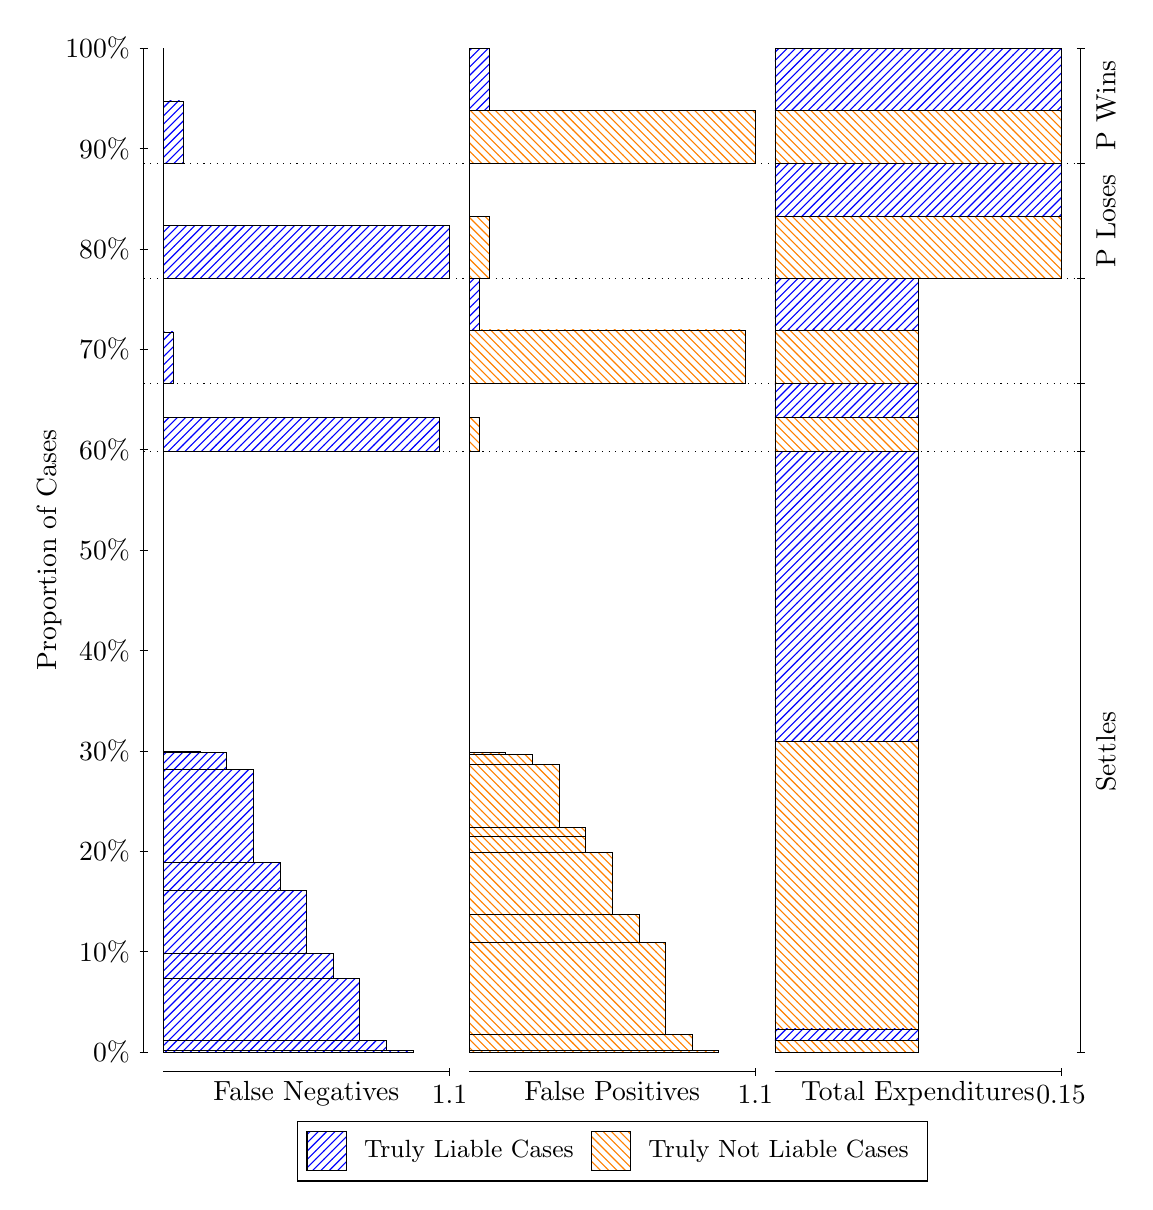
\begin{tikzpicture}
\draw[black, very thin] (1.5,1.75) -- (1.5,14.5);
\node[rotate=90, anchor=center] at (0.3, 8.125) {Proportion of Cases};
\draw[black, very thin] (1.45,1.75) -- (1.55,1.75);
\node[anchor=east] at (1.45, 1.75) {0\%};
\draw[black, very thin] (1.45,3.025) -- (1.55,3.025);
\node[anchor=east] at (1.45, 3.025) {10\%};
\draw[black, very thin] (1.45,4.3) -- (1.55,4.3);
\node[anchor=east] at (1.45, 4.3) {20\%};
\draw[black, very thin] (1.45,5.575) -- (1.55,5.575);
\node[anchor=east] at (1.45, 5.575) {30\%};
\draw[black, very thin] (1.45,6.85) -- (1.55,6.85);
\node[anchor=east] at (1.45, 6.85) {40\%};
\draw[black, very thin] (1.45,8.125) -- (1.55,8.125);
\node[anchor=east] at (1.45, 8.125) {50\%};
\draw[black, very thin] (1.45,9.4) -- (1.55,9.4);
\node[anchor=east] at (1.45, 9.4) {60\%};
\draw[black, very thin] (1.45,10.675) -- (1.55,10.675);
\node[anchor=east] at (1.45, 10.675) {70\%};
\draw[black, very thin] (1.45,11.95) -- (1.55,11.95);
\node[anchor=east] at (1.45, 11.95) {80\%};
\draw[black, very thin] (1.45,13.225) -- (1.55,13.225);
\node[anchor=east] at (1.45, 13.225) {90\%};
\draw[black, very thin] (1.45,14.5) -- (1.55,14.5);
\node[anchor=east] at (1.45, 14.5) {100\%};

\draw[black, very thin] (13.4,1.75) -- (13.4,14.5);
\draw[black, very thin] (13.35,1.75) -- (13.45,1.75);
\node[anchor=west] at (13.35, 1.75) {};
\draw[black, very thin] (13.35,9.3737) -- (13.45,9.3737);
\node[anchor=west] at (13.35, 9.3737) {};
\draw[black, very thin] (13.35,10.242) -- (13.45,10.242);
\node[anchor=west] at (13.35, 10.242) {};
\draw[black, very thin] (13.35,11.573) -- (13.45,11.573);
\node[anchor=west] at (13.35, 11.573) {};
\draw[black, very thin] (13.35,13.036) -- (13.45,13.036);
\node[anchor=west] at (13.35, 13.036) {};
\draw[black, very thin] (13.35,14.5) -- (13.45,14.5);
\node[anchor=west] at (13.35, 14.5) {};

\draw[black, very thin, pattern color=blue, pattern=north east lines] (1.75,1.75) rectangle (4.9186,1.7739);
\draw[black, very thin, pattern color=blue, pattern=north east lines] (1.75,1.7739) rectangle (4.5806,1.8928);
\draw[black, very thin, pattern color=blue, pattern=north east lines] (1.75,1.8928) rectangle (4.2426,2.689);
\draw[black, very thin, pattern color=blue, pattern=north east lines] (1.75,2.689) rectangle (3.9047,3.0018);
\draw[black, very thin, pattern color=blue, pattern=north east lines] (1.75,3.0018) rectangle (3.5667,3.7992);
\draw[black, very thin, pattern color=blue, pattern=north east lines] (1.75,3.7992) rectangle (3.2287,4.1587);
\draw[black, very thin, pattern color=blue, pattern=north east lines] (1.75,4.1587) rectangle (2.8907,5.3423);
\draw[black, very thin, pattern color=blue, pattern=north east lines] (1.75,5.3423) rectangle (2.5527,5.5506);
\draw[black, very thin, pattern color=blue, pattern=north east lines] (1.75,5.5506) rectangle (2.2147,5.5722);
\draw[black, very thin, pattern color=orange, pattern=north west lines] (1.75,5.5722) rectangle (1.75,9.3737);
\draw[black, very thin, pattern color=blue, pattern=north east lines] (1.75,9.3737) rectangle (5.2566,9.8077);
\draw[black, very thin, pattern color=orange, pattern=north west lines] (1.75,9.8077) rectangle (1.75,10.242);
\draw[black, very thin, pattern color=blue, pattern=north east lines] (1.75,10.242) rectangle (1.8767,10.895);
\draw[black, very thin, pattern color=orange, pattern=north west lines] (1.75,10.895) rectangle (1.75,11.573);
\draw[black, very thin, pattern color=blue, pattern=north east lines] (1.75,11.573) rectangle (5.3833,12.246);
\draw[black, very thin, pattern color=orange, pattern=north west lines] (1.75,12.246) rectangle (1.75,13.036);
\draw[black, very thin, pattern color=blue, pattern=north east lines] (1.75,13.036) rectangle (2.0035,13.829);
\draw[black, very thin, pattern color=orange, pattern=north west lines] (1.75,13.829) rectangle (1.75,14.5);
\draw[black, very thin, pattern color=orange, pattern=north west lines] (5.6333,1.75) rectangle (8.8019,1.7718);
\draw[black, very thin, pattern color=orange, pattern=north west lines] (5.6333,1.7718) rectangle (8.464,1.9764);
\draw[black, very thin, pattern color=orange, pattern=north west lines] (5.6333,1.9764) rectangle (8.126,3.1446);
\draw[black, very thin, pattern color=orange, pattern=north west lines] (5.6333,3.1446) rectangle (7.788,3.4976);
\draw[black, very thin, pattern color=orange, pattern=north west lines] (5.6333,3.4976) rectangle (7.45,4.2859);
\draw[black, very thin, pattern color=orange, pattern=north west lines] (5.6333,4.2859) rectangle (7.112,4.4859);
\draw[black, very thin, pattern color=orange, pattern=north west lines] (5.6333,4.4859) rectangle (7.112,4.6001);
\draw[black, very thin, pattern color=orange, pattern=north west lines] (5.6333,4.6001) rectangle (6.774,5.401);
\draw[black, very thin, pattern color=orange, pattern=north west lines] (5.6333,5.401) rectangle (6.436,5.5257);
\draw[black, very thin, pattern color=orange, pattern=north west lines] (5.6333,5.5257) rectangle (6.0981,5.5515);
\draw[black, very thin, pattern color=blue, pattern=north east lines] (5.6333,5.5515) rectangle (5.6333,9.3737);
\draw[black, very thin, pattern color=orange, pattern=north west lines] (5.6333,9.3737) rectangle (5.7601,9.8077);
\draw[black, very thin, pattern color=blue, pattern=north east lines] (5.6333,9.8077) rectangle (5.6333,10.242);
\draw[black, very thin, pattern color=orange, pattern=north west lines] (5.6333,10.242) rectangle (9.1399,10.92);
\draw[black, very thin, pattern color=blue, pattern=north east lines] (5.6333,10.92) rectangle (5.7601,11.573);
\draw[black, very thin, pattern color=orange, pattern=north west lines] (5.6333,11.573) rectangle (5.8868,12.363);
\draw[black, very thin, pattern color=blue, pattern=north east lines] (5.6333,12.363) rectangle (5.6333,13.036);
\draw[black, very thin, pattern color=orange, pattern=north west lines] (5.6333,13.036) rectangle (9.2667,13.708);
\draw[black, very thin, pattern color=blue, pattern=north east lines] (5.6333,13.708) rectangle (5.8868,14.5);
\draw[black, very thin, pattern color=orange, pattern=north west lines] (9.5167,1.75) rectangle (11.333,1.9005);
\draw[black, very thin, pattern color=blue, pattern=north east lines] (9.5167,1.9005) rectangle (11.333,2.0433);
\draw[black, very thin, pattern color=orange, pattern=north west lines] (9.5167,2.0433) rectangle (11.333,5.6943);
\draw[black, very thin, pattern color=blue, pattern=north east lines] (9.5167,5.6943) rectangle (11.333,9.3737);
\draw[black, very thin, pattern color=orange, pattern=north west lines] (9.5167,9.3737) rectangle (11.333,9.8077);
\draw[black, very thin, pattern color=blue, pattern=north east lines] (9.5167,9.8077) rectangle (11.333,10.242);
\draw[black, very thin, pattern color=orange, pattern=north west lines] (9.5167,10.242) rectangle (11.333,10.92);
\draw[black, very thin, pattern color=blue, pattern=north east lines] (9.5167,10.92) rectangle (11.333,11.573);
\draw[black, very thin, pattern color=orange, pattern=north west lines] (9.5167,11.573) rectangle (13.15,12.363);
\draw[black, very thin, pattern color=blue, pattern=north east lines] (9.5167,12.363) rectangle (13.15,13.036);
\draw[black, very thin, pattern color=orange, pattern=north west lines] (9.5167,13.036) rectangle (13.15,13.708);
\draw[black, very thin, pattern color=blue, pattern=north east lines] (9.5167,13.708) rectangle (13.15,14.5);
\draw[black, dotted] (1.5,9.3737) -- (13.4,9.3737);
\draw[black, dotted] (1.5,10.242) -- (13.4,10.242);
\draw[black, dotted] (1.5,11.573) -- (13.4,11.573);
\draw[black, dotted] (1.5,13.036) -- (13.4,13.036);
\draw[black, very thin] (1.75,1.5) -- (5.3833,1.5);
\node[anchor=north] at (3.5667, 1.5) {False Negatives};
\draw[black, very thin] (5.3833,1.45) -- (5.3833,1.55);
\node[anchor=north] at (5.3833, 1.45) {1.1};

\draw[black, very thin] (5.6333,1.5) -- (9.2667,1.5);
\node[anchor=north] at (7.45, 1.5) {False Positives};
\draw[black, very thin] (9.2667,1.45) -- (9.2667,1.55);
\node[anchor=north] at (9.2667, 1.45) {1.1};

\draw[black, very thin] (9.5167,1.5) -- (13.15,1.5);
\node[anchor=north] at (11.333, 1.5) {Total Expenditures};
\draw[black, very thin] (13.15,1.45) -- (13.15,1.55);
\node[anchor=north] at (13.15, 1.45) {0.15};

\node[black, centered, rotate=90] at (13.72, 5.5619) {Settles};


\node[black, centered, rotate=90] at (13.72, 12.305) {P Loses};
\node[black, centered, rotate=90] at (13.72, 13.768) {P Wins};

\draw (7.449999999999999,1.5) node[draw=none] (baseCoordinate) {};
\begin{scope}[align=center]
        \matrix[scale=0.5, draw=black, below=0.5cm of baseCoordinate, nodes={draw}, column sep=0.1cm]{
            \node[rectangle, draw, minimum width=0.5cm, minimum height=0.5cm, pattern=north east lines, pattern color=blue] {}; &
            \node[draw=none, font=\small] (B) {Truly Liable Cases}; &
            \node[rectangle, draw, minimum width=0.5cm, minimum height=0.5cm, pattern=north west lines, pattern color=orange] {}; &
            \node[draw=none, font=\small] (B) {Truly Not Liable Cases}; \\
            };
\end{scope}

\end{tikzpicture}
\end{document}